\documentclass[../pde_notes.tex]{subfiles}
\begin{document}
\section{Aula 09 - 31 de Março, 2025}
\subsection{Motivações}
\begin{itemize}
	\item Convergência das Séries de Fourier.
\end{itemize}
\subsection{Convergência das Séries de Fourier}
Considere a função \(f:\mathbb{R}\rightarrow \mathbb{C}\), \(2\pi \)-periódica, com a seguinte forma se escrever sua série de Fourier:
\begin{align*}
	 & f(x)=\lim_{N\to \infty}\sum\limits_{n=-N}^{N}c_{n}e^{inx} = \lim_{N\to \infty}\biggl[\frac{a_{0}}{2}+\sum\limits_{n=1}^{N}(a_{n})\cos^{}{(nx)}+b_{n}\sin^{}{(nx)}\biggr] \\
	 & c_{n}=\frac{1}{2\pi }\int_{-\pi }^{\pi }f(x)e^{-inx}dx.
\end{align*}
Nosso tópico de discussão dessa vez tem relação com o termo que vem logo antes da série descrita acima: o limite; mais especificamente, a convergência das séries de Fourier. Iremos passar pela convergência pontual, que diz respeito à convergência de uma função em cada ponto, pela uniforme, sobre a convergência ser controlada para todos os pontos do domínio dela, e algumas outras, como a \(L^{2}\). Para uma especificidade maior, a pontual significa que, para cada x dentro de um subconjunto dos reais,
\[
	f(x)=\lim_{N\to \infty}\sum\limits_{n=-N}^{N}c_{n}e^{inx}.
\]
Por outro lado, a uniforme assumiria a forma da igualdade
\[
	\lim_{N\to \infty}\max_{x\in \mathbb{R}}\biggl\vert f(x)-\sum\limits_{n=-N}^{N}c_{n}e^{inx} \biggr\vert=0,
\]
e, a \(L^{2}\),
\[
	\lim_{N\to \infty}\int_{-\pi }^{\pi }\biggl\vert f(x)-\sum\limits_{n=-N}{N}c_{n}e^{inx} \biggr\vert^{2} dx = 0.
\]
Dizer que elas são fáceis de checar é um exagero, então elas serão parte dos principais tópicos de estudo dessa parte.

Antes, porém, definimos
\begin{def*}
	Uma função \(f:[a, b]\rightarrow \mathbb{R}\) é \textbf{contínua por partes} se existe uma \textit{partição} do intervalo \([a, b]\)
	\[
		a=x_{0}<x_{1}<\dotsc <x_{n}=b
	\]
	tal que
	\begin{itemize}
		\item[1)] A restrição de f aos subintervalos gerados pela partição, ou seja,
		      \[
			      f|_{(x_{i}, x_{i+1})},
		      \]
		      é contínua;
		\item[2)] Existem os limites laterais para cada componente da partição, isto é,
		      \[
			      \lim_{x\to x_{i}^{+}}f(x)\quad\&\quad \lim_{x\to x_{i}^{-}}f(x).\quad \square
		      \]
	\end{itemize}
\end{def*}
\begin{figure}[H]
	\begin{center}
		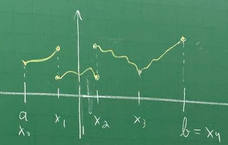
\includegraphics[height=0.6\textheight, width=0.6\textwidth, keepaspectratio]{./Images/squiggles_09.png}
	\end{center}
	\caption{ilustração da continuidade por partes - um monte de ``componentes contínuas'' da função em cada parte da partição.}
	\label{sqgl09}
\end{figure}

\begin{example}
	\begin{itemize}
		\item[a)] A função
		      \[
			      f(x) = \left\{\begin{array}{ll}
				      \frac{1}{x}, & \quad x\in (0, 1] \\
				      0,           & \quad x=0
			      \end{array}\right.
		      \]
		      não é contínua por partes - ela falha quando olhamos para qualquer partição em seus componentes \(a=x_{0}=0\) e \(x_{1}>0\)
		\item[b)] Similarmente, a função
		      \[
			      f(x) = \left\{\begin{array}{ll}
				      \sin^{}{\biggl(\frac{1}{x}\biggr)}, & \quad x\in (0, 1]  \\
				      0,                                  & \quad x\in [-1, 0]
			      \end{array}\right.
		      \]
		      também não é.
		\item[c)] Finalmente, um exemplo de função contínua por partes é
		      \[
			      f(x) = \left\{\begin{array}{ll}
				      x,   & \quad x\in [0,1]   \\
				      1+x, & \quad x\in [-1, 0]
			      \end{array}\right.
		      \]
	\end{itemize}
\end{example}
\begin{def*}
	Uma função \(f:[a, b]\rightarrow \mathbb{R}\) é \(\mathcal{C}^{1}\)\textbf{ por partes}, ou \textbf{suave por partes}\footnote{O termo suave sempre tem que ser levado com cautela. Em geral, suave significa ter todas as derivadas contínuas, mas, muitas vezes, pode ser usado para se referir à derivada conveniente ser contínua. No caso daqui, basta que a primeira seja, então suave significa uma função ter derivada e ela ser contínua.}, se existe uma \textit{partição} do intervalo \([a, b]\)
	\[
		a=x_{0}<x_{1}<\dotsc <x_{n}=b
	\]
	tal que
	\begin{itemize}
		\item[1)] A restrição de f aos subintervalos gerados pela partição, ou seja,
		      \[
			      f|_{(x_{i}, x_{i+1})},
		      \]
		      é \(\mathcal{C}^{1}\);
		\item[2)] Existem os limites laterais da função e de sua derivada para cada componente da partição, isto é,
		      \[
			      \lim_{x\to x_{i}^{+}}f(x),\: \lim_{x\to x_{i}^{-}}f(x),\: \lim_{x\to x_{i}^{+}}f'(x) \:\&\: \lim_{x\to x_{i}^{-}}f'(x).\quad \square
		      \]
	\end{itemize}
\end{def*}
\begin{figure}[H]
	\begin{center}
		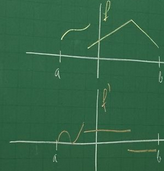
\includegraphics[height=0.6\textheight, width=0.6\textwidth, keepaspectratio]{./Images/lines_09.png}
	\end{center}
	\caption{de forma parecida com a anterior, temos a ilustração de uma função \(\mathcal{C}^{1}\) por partes.}
	\label{lines09}
\end{figure}
É preciso ter cautela ao afirmar que uma função é \(\mathcal{C}^{1}\) por partes apenas por suas propriedades; a exemplo, a função
\[
	f(x) = \left\{\begin{array}{ll}
		\sqrt[]{x}, & \quad x\in [0,1]   \\
		0,          & \quad x\in [-1, 0]
	\end{array}\right.
\]
é contínua, MAS não é \(\mathcal{C}^{1}\) por partes: basta ver sua primeira derivada e comparar com o exemplo (a) das funções que não são contínuas por partes.

\begin{def*}
	Uma função \(f:\mathbb{R}\rightarrow \mathbb{C}\) é \textbf{contínua (suave) por partes} se, para cada \(a<b\), as suas partes real e imaginária ,
	\[
		\mathrm{Re}(f):[a, b]\rightarrow \mathbb{R} \quad\&\quad \mathrm{Im}(f):[a, b]\rightarrow \mathbb{R}
	\]
	são contínuas (suaves) por partes. \(\square\)
\end{def*}
Observe que, caso ela seja \(2\pi \)-periódica, bastaria provar para o intervalo \([-\pi , \pi ]\).
\begin{tcolorbox}[
		skin=enhanced,
		title=Lembrete!,
		after title={\hfill Parte Real e Imaginária},
		fonttitle=\bfseries,
		sharp corners=downhill,
		colframe=black,
		colbacktitle=yellow!75!white,
		colback=yellow!30,
		colbacklower=black,
		coltitle=black,
		%drop fuzzy shadow,
		drop large lifted shadow
	]
	Quando temos uma função com codomínio complexo, \(f:X\rightarrow Y\subseteq \mathbb{C}\), ela pode ser escrita como
	\[
		f(x, y)=u(x, y)+iv(x, y),
	\]
	de forma análoga aos próprios números complexos, com forma
	\[
		z = x+iy.
	\]
	A analogia vai um pouco além: da mesma forma que a parte real de z é x, e a imaginária é y (sem o i), temos as partes real e imaginária de f como
	\[
		\mathrm{Re}(f)=u(x, y) \quad\&\quad \mathrm{Im}(f)=v(x, y).
	\]
\end{tcolorbox}
\hypertarget{ponintwise_convergence}{\begin{theorem*}[Convergência Pontual das Séries de Fourier]
		Seja \(f:\mathbb{R}\rightarrow \mathbb{C}\) uma função \(2\pi \)-periódica e \(\mathcal{C}^{1}\) por partes. Então,
		\[
			\lim_{N\to \infty}\sum\limits_{n=-N}^{N}c_{n}e^{inx}=\lim_{N\to \infty}\frac{a_{0}}{2}+\sum\limits_{n=1}^{N}(a_{n}\cos^{}{(nx)}+b_{n}\sin^{}{(nx)})=\frac{f(x^{+})+f(x^{-})}{2},
		\]
		em que as funções na divisão representam, respectivamente, os limites laterais da f:
		\[
			f(x_{0}^{+})\coloneqq \lim_{x\to x_{0}^{+}}f(x),\quad f(x_{0}^{-})=\lim_{x\to x_{0}^{-}}f(x).
		\]
	\end{theorem*}}
A prova deste teorema pode ser vista como composta por dois passos: a desigualdade de Bessel e o estudo do núcleo de Dirichlet
\hypertarget{bessel_inequality}{
	\begin{prop*}[Desigualdade de Bessel]
		Seja \(g:\mathbb{R}\rightarrow \mathbb{C}\) contínua por partes e
		\[
			c_{N}=\frac{1}{2\pi }\int_{-\pi }^{\pi }g(x)e^{-inx}dx.
		\]
		Então,
		\[
			\lim_{N\to \infty}\sum\limits_{n=-N}^{N}|c_{n}|^{2}=\sum\limits_{n=-\infty}^{\infty}|c_{n}|^{2}\leq \frac{1}{2\pi }\int_{-\pi }^{\pi }|g(x)|^{2}dx.
		\]
	\end{prop*}
}
\begin{proof*}[Ideia]
	A ideia dessa prova é utilizar conceitos de álgebra linear: ao considerar uma base ortonormal \(\mathcal{B}=\{e_{1},\dotsc ,e_{n}\}\), ou seja, uma base tal que
	\[
		\left< e_{i}, e_{j} \right>=\delta_{ij},
	\]
	então podemos escrever
	\[
		u=\left< u, e_{1} \right>e_{1}+\dotsc + \left< u, e_{n} \right>e_{n}.
	\]
	Assim,
	\[
		\Vert u \Vert^{2}=\sum\limits_{j=1}^{n}|\left< u, e_{j} \right>|^{2}.
	\]
	No nosso caso,
	\[
		u=\sum\limits_{n=-\infty}^{\infty}\frac{c_{n}}{2\pi }\biggl\{\frac{1}{\sqrt[]{2\pi }}e^{inx}\biggr\},
	\]
	tal que, com \(e_{n}\) sendo o termo em parênteses,
	\[
		\Vert u \Vert^{2}=\sum\limits_{n=-\infty}^{\infty}\frac{|c_{n}|^{2}}{2\pi }.
	\]
	A partir disso, sabemos que
	\[
		\biggl\Vert g(x)-\sum\limits_{n=-N}^{N}c_{n}e^{inx} \biggr\Vert^{2}\geq 0
	\]
	e, usando a definição de norma como
	\[
		\Vert h \Vert^{2}=\left< h, h \right>=\int_{-\pi }^{\pi }|h(x)|^{2}dx,
	\]
	podemos reescrever a desigualdade acima com a cara
	\[
		\int_{-\pi }^{\pi }|g(x)-\sum\limits_{n=-N}^{N}c_{n}e^{inx}|^{2}dx\geq 0.
	\]
	Como estamos mexendo com números complexos, o módulo pode ser visto como um produto do termo dentro dele pelo seu conjugado complexo, tal que
	\begin{align*}
		0 & \leq \int_{-\pi }^{\pi }\biggl(g(x)-\sum\limits_{n=-N}^{N}c_{n}e^{inx}\biggr)\biggl(\overline{g(x)}-\sum\limits_{m=-N}^{N}\overline{c_{m}}e^{-imx}\biggr)dx                                                                                                                                      \\
		\\
		  & =\int_{-\pi }^{\pi }|g(x)|^{2}dx - \underbrace{\sum\limits_{m=-N}^{N}\overline{c_{m}}\int_{-\pi }^{\pi }g(x)e^{-inx}dx}_{2\pi \sum\limits_{m=-N}^{N}|c_{m}|^{2}} - \underbrace{\overline{\sum\limits_{n=-N}^{N}c_{n}\int_{-\pi }^{\pi }g(x)e^{-inx}dx}}_{2\pi \sum\limits_{n=-N}^{N}|c_{n}|^{2}} \\
		  & +\sum\limits_{n=-N}^{N}\sum\limits_{m=-N}^{N}c_{n}\overline{c_{m}}\underbrace{\int_{-\pi }^{\pi }e^{i(n-m)x}dx}_{2\pi \delta_{nm}}                                                                                                                                                               \\
		\\
		  & = \int_{-\pi }^{\pi }|g(x)|^{2}dx + (-2\pi - 2\pi + 2\pi)\sum\limits_{n=-N}^{N}|c_{n}|^{2}.
	\end{align*}
	Portanto,
	\[
		0\leq \int_{-\pi }^{\pi }|g(x)|^{2}dx - 2\pi \sum\limits_{n=-N}^{N}|c_{n}|^{2}.\quad \text{\qedsymbol}
	\]
\end{proof*}
Podemos ir ao passo 2 agora, relacionado ao núcleo de Dirichlet.
\begin{prop*}
	Seja \(g:\mathbb{R}\rightarrow \mathbb{C}\) uma função \(2\pi\)-periódica e contínua por partes. Então,
	\begin{align*}
		 & \sum\limits_{n=-N}^{N}c_{n}e^{inx}=\int_{-\pi }^{\pi }D_{n}(x-y)g(y)dy \\
		 & c_{n}=\frac{1}{2\pi }\int_{-\pi }^{\pi }g(y)e^{-iny}dy,
	\end{align*}
	em  que
	\[
		D_{N}(x)\coloneqq \frac{1}{2\pi }\sum\limits_{n=-N}^{N}e^{inx}.
	\]
\end{prop*}
\begin{proof*}
	Basta fazer uma conta e obtemos
	\[
		\sum\limits_{n=-N}^{N}\biggl(\frac{1}{2\pi }\int_{-\pi }^{\pi }g(y)e^{-iny}dy\biggr)e^{inx}=\int_{-\pi }^{\pi }\biggl(\frac{1}{2\pi }\sum\limits_{n=-N}^{N}e^{in(x-y)}\biggr)g(y)dy=D_{N}(x-y).\quad \text{\qedsymbol}
	\]
\end{proof*}
O valor \(D_{N}\) é chamado \textbf{núcleo de Dirichlet}.
\begin{prop*}
	Vale a igualdade
	\[
		D_{N}(x)=\frac{1}{2\pi }\frac{e^{-iNx}-e^{i(N+1)x}}{1-e^{ix}} \quad\&\quad \int_{-\pi }^{0}D_{N}(x)dx=\int_{0}^{\pi }D_{N}(x)dx=\frac{1}{2}.
	\]
\end{prop*}
\begin{proof*}
	Basta observar que
	\begin{align*}
		2\pi D_{N}(x)=\sum\limits_{n=-N}^{N}e^{inx} & =\sum\limits_{m=0}^{2N}e^{i(m-N)x}          \\
		                                            & =e^{-iNx}\sum\limits_{m=0}^{2N}e^{imx}      \\
		                                            & =e^{-iNx}\sum\limits_{m=0}^{2N}(e^{ix})^{m} \\
		                                            & =e^{-iNx}\frac{1-e^{i(2N+1)x}}{1-e^{ix}}    \\
		                                            & =\frac{e^{-iNx}-e^{i(N+1)x}}{1-e^{ix}}.
	\end{align*}
	Quanto aos valores especificados da integral, partimos de
	\[
		2\pi D_{N}(x)=1+\sum\limits_{n=-N}^{-1}e^{inx}+\sum\limits_{n=1}^{N}e^{inx}=1+\sum\limits_{n=1}^{N}e^{-inx}+\sum\limits_{n=1}^{N}e^{inx}=1+2\sum\limits_{n=1}^{N}\cos^{}{(nx)}.
	\]
	Logo,
	\begin{align*}
		 & 2\pi \int_{-\pi }^{0}D_{N}(x)dx=\int_{-\pi }^{0}\biggl(1+2\sum\limits_{n=1}^{N}\cos^{}{(nx)}\biggr)dx = \pi -2\sum\limits_{n=1}^{N}\frac{\sin^{}{(nx)}}{n}\biggl|_{-\pi }^{0}\biggr.=\pi   \\
		 & 2\pi \int_{0}^{\pi }D_{N}(x)dx=\int_{0}^{\pi}\biggl(1+2\sum\limits_{n=1}^{N}\cos^{}{(nx)}\biggr)dx = \pi -2\sum\limits_{n=1}^{N}\frac{\sin^{}{(nx)}}{n}\biggl|_{0}^{\pi}\biggr.=\pi      .
	\end{align*}
	Portanto, dividindo ambos por \(2\pi \), obtemos
	\begin{align*}
		 & \int_{-\pi}^{0}D_{N}(x)dx=\frac{1}{2}       \\
		 & \int_{0}^{\pi }D_{N}(x)dx=\frac{1}{2}     .
	\end{align*}
\end{proof*}
Agora sim, podemos provar o \hyperlink{ponintwise_convergence}{\textit{teorema da convergência pontual}}.
\begin{proof*}[Convergência Pontual]
	Primeiramente, observe que, colocando \(\tilde{y}=x-y\),
	\[
		\int_{-\pi }^{\pi }D_{N}(x-y)f(y)dy=\int_{x-\pi }^{x+\pi }D_{N}(\tilde{y})f(x-\tilde{y})d\tilde{y}.
	\]
	Em seguida, note que, colocando
	\[
		F'(a)=\int_{a-\pi }^{a+\pi }g(x)dx=g(a+\pi )-g(a-\pi )=0,
	\]
	então F(a) é constante e
	\[
		F(a)=F(0) \Rightarrow \int_{a-\pi }^{a+\pi }g(x)dx=\int_{-\pi }^{\pi }g(x)dx.
	\]
	Logo,
	\[
		\int_{x-\pi }^{x+\pi }D_{N}(\tilde{y})f(x-\tilde{y})d\tilde{y}=\int_{-\pi }^{\pi }D_{N}(y)f(x-y)dy.
	\]
	Fizemos isto pois esta integral tornar-se-á o valor da função à esquerda e à direita. Desta forma,
	\begin{align*}
		 & \sum\limits_{n=-N}^{N}-\frac{f(x^{+})-f(x^{-})}{2}                                                                                                                                   \\
		 & = \sum\limits_{n=-N}^{N}-{\color{red}\frac{f(x^{+})}{2}}-{\color{green}\frac{f(x^{-})}{2}}                                                                                           \\
		 & =\int_{-\pi }^{\pi }D_{N}(y)f(x-y)dy - {\color{red}\int_{-\pi }^{0}f(x^{+})D_{N}(y)dy}-{\color{green}\int_{0}^{\pi }f(x^{-})D_{N}(y)dy}                                              \\
		 & = \int_{0}^{\pi }D_{N}(y)(f(x-y)-f(x^{-}))dy + \int_{-\pi }^{0}D_{N}(y)(f(x-y)-f(x^{+}))dy                                                                                           \\
		 & = \int_{0}^{\pi }\frac{1}{2 \pi }(e^{-iNy}-e^{i(N+1)y})\frac{f(x-y)-f(x^{-})}{1-e^{iy}}dy + \int_{-\pi }^{0}\frac{1}{2\pi }(e^{-iNy}-e^{i(N+1)y})\frac{f(x-y)-f(x^{+})}{1-e^{iy}}dy.
	\end{align*}
	Com isso, definindo
	\[
		g_{x}(y) = \left\{\begin{array}{ll}
			\frac{f(x-y)-f(x^{-})}{1-e^{iy}}, & \quad y\in [0, \pi ] \\
			\frac{f(x-y)-f(x^{+})}{1-e^{iy}}, & \quad y\in [-\pi, 0]
		\end{array}\right.
	\]
	para colocar os mesmos limites de integração nas duas integrais integral e
	\[
		d_{n}=\frac{1}{2\pi }\int_{-\pi }^{\pi }g_{x}(y)e^{-iny}dy,
	\]
	tal que
	\[
		\sum\limits_{n=-\infty}^{\infty}|d_{n}|^{2}\leq 2\pi \int_{-\pi }^{\pi }|g_{x}(y)|^{2}dy \Rightarrow \lim_{N\to \infty}d_{n}=0.
	\]
	Temos, portanto,
	\begin{align*}
		 & \int_{0}^{\pi }\frac{1}{2 \pi }(e^{-iNy}-e^{i(N+1)y})\frac{f(x-y)-f(x^{-})}{1-e^{iy}}dy + \int_{-\pi }^{0}\frac{1}{2\pi }(e^{-iNy}-e^{i(N+1)y})\frac{f(x-y)-f(x^{+})}{1-e^{iy}}dy \\
		 & = \frac{1}{2\pi } \int_{-\pi }^{\pi }e^{-iNy}g_{x}(y)dy - \frac{1}{2\pi }\int_{-\pi }^{\pi }e^{i(N+1)y}g_{x}(y)dy                                                                 \\
		 & =d_{N}-d_{-(N+1)} \overbracket[0pt]{\longrightarrow}^{N\to \infty}0. \quad \text{\qedsymbol}
	\end{align*}
\end{proof*}
Na aula seguinte, mostraremos que a função \(g_{x}:\mathbb{R}\rightarrow \mathbb{C}\) é contínua por partes.
\end{document}
